% Created 2021-04-08 Thu 22:26
% Intended LaTeX compiler: pdflatex
\documentclass[11pt]{article}
\usepackage[utf8]{inputenc}
\usepackage[T1]{fontenc}
\usepackage{graphicx}
\usepackage{grffile}
\usepackage{longtable}
\usepackage{wrapfig}
\usepackage{rotating}
\usepackage[normalem]{ulem}
\usepackage{amsmath}
\usepackage{textcomp}
\usepackage{amssymb}
\usepackage{capt-of}
\usepackage{hyperref}
\author{Fabio Favero Henkes}
\date{\today}
\title{}
\hypersetup{
 pdfauthor={Fabio Favero Henkes},
 pdftitle={},
 pdfkeywords={},
 pdfsubject={},
 pdfcreator={Emacs 26.1 (Org mode 9.1.9)},
 pdflang={English}}
\begin{document}

\tableofcontents

\section{PAX RENAISSANCE (2 jogadores)}
\label{sec:org5df7bc0}

\subsection{AÇÕES (2 por turno)}
\label{sec:orgc25efa2}

\subsubsection{COMPRAR UMA CARTA}
\label{sec:orgd9779e8}

Coloque uma carta do mercado em sua mão. Adicione 1 Florin para cada carta na mesma linha à esquerda da carta que estiver comprando (ou na outra linha, caso alguma carta esteja faltando).
Pegue qualquer quantidade de Florins que estiverem por ventura na carta que foi comprada.

\begin{itemize}
\item Se vc colocar um Florin em uma determinada carta do mercado, não pode mais comprá-la esse turno (na sua próxima ação).

\item Nunca é possível ter mais que 2 cartas na mão.
\end{itemize}

\subsubsection{JOGANDO UMA CARTA DA MÃO E COLOCANDO AGENTES}
\label{sec:org87a761c}

Baixe uma carta da sua mão em seu Tableau, de acordo com a orientação da carta (leste ou oeste).

Caso a carta jogada tiver um ícone de bomba, deve-se primeiramente decidir se o evento \emph{one-shot} ocorre.

A colocação de agentes é opcional, pode-se colocar todos, alguns ou nenhum deles.

Exceção: No caso de o \emph{one-shot} ser uma guerra, civil ou religiosa, deve-se obrigatóriamente colocar os agentes Cavalo, Torre e/ou Peões como atacantes na batalha.

\begin{itemize}
\item Se for colocado um Cavalo, Torre ou Peão onde já houver outro agente (não pirata), este deve ser reprimido pelo valor de 1 Florin.

\item Se for adicionado um pirata onde já existir um outro pirata ou mercador, mate-o de graça (peça volta para o estoque).
\end{itemize}

\subsubsection{VENDER UMA CARTA}
\label{sec:org1ff5166}

Descarte uma carta de sua mão ou de seu Tableau e ganhe 2 Florins.

\subsubsection{EXECUTAR OPERAÇÕES (LESTE/OESTE)}
\label{sec:org065e4a9}

No máximo uma vez por turno é possível executar uma operação em cada carta de seu Tableau em determinado sentido (leste/oeste), em qualquer ordem que desejar.

\subsubsection{PERCORRA A ROTA COMERCIAL (LESTE/OESTE)}
\label{sec:orge32c7d5}

No máximo uma vez por turno é possível percorrer uma das rotas comerciais a sua escolha. Adicione 1 Florin (2 jogadores) do Banco (China) à carta virada para baixo no ínicio do mercado escolhido.

O total de Florins existente na carta é chamado Lucro.

O jogador que iniciou a rota (escolheu essa ação) recebe 1 Florin.

Trace a rota desejada a partir do seu início, dependendo de qual delas (linha preta/leste ou branca/oeste), um ponto não bloqueado (rota atual).

Todos os mercadores ao longo da rota recebem 1 Florin cada até que o lucro termine.

\begin{itemize}
\item Caso haja um pirata na rota o Florin é descartado para o banco (China).

\item Caso acabarem os Florins a rota para imediatamente.

\item Cada carta pela qual a rota atravessou faz um recrutamento (Levy), um token de Cavalo ou Torre é adicionado caso haja espaço na carta à escolha do jogador, a cor deve bater com o ícone na carta.

\item Caso a rota tenha acabado antes do final, as cartas que não foram alcançadas pela rota não realizam recrutamento.

\item Descarte a carta do mercado (leste ou oeste) virada para baixo

\item Vire a primeira carta do mercado, puxe o "comboio" de cartas e adicione uma nova carta ao final.

\item Caso reste Lucro (sobrem Florins sobre a carta virada), estes permanecem na nova carta que será virada no início do  mercado.
\end{itemize}

\subsubsection{AÇÃO DE VITÓRIA}
\label{sec:org1284833}

Use esta ação para declarar vitória, baseada em uma das cartas de vitória \textbf{ATIVAS}.

\begin{itemize}
\item \textbf{Vitória Religiosa}: para vencer é necessário obter maior prestígio na religião predominante no mapa que seu oponente. A religião é considerada predominante quando:
\begin{itemize}
\item Possuir mais bispos de sua cor em jogo do que as duas outras religiões combinadas;
\item Possuir mais tokens (Cavaleiros, Torres e Piratas) de sua cor em jogo nas suas teocracias do que as duas outras regiões combinadas.
\end{itemize}

\item \textbf{Vitória Imperial}: para vencer é necessário obter pelo menos mais 3 cartas de Império que seu oponente (2 jogadores). Não importa se Suseranos ou Vassalos.

\item \textbf{Vitória por Globalização}: para vencer é preciso obter dois ou mais mercadores a mais que seu oponente e mais ícones de prestígio de Descoberta.

\item \textbf{Vitória Renascentista}: para vencer é preciso obter mais repúblicas que seu oponente e ter pelo menos dois ícones de prestígio de Lei a mais que seu oponente.

\item \textbf{Vitória Burguesa}: o jogo acaba se os dois decks, leste e oeste forem esvaziados durante o \emph{refresh} do mercado. Caso isso ocorra o jogador com mais prestígio de Burguesia (Patron) vence.
\end{itemize}
Em caso de empate a vitória vai para àquele com mais Florins.


\subsection{GLOSSÁRIO}
\label{sec:orgd66b3f6}

\subsubsection{BATALHA}
\label{sec:org7a7a144}

Para resolver uma Campanha, Guerra Civil ou Guerra Religiosa, cada token atacante mata umm token defensor, mas é também morto em troca. O jogador atacante escolhe as baixas.

Os tokes atacantes são vitoriosos caso tenham ao menos um sobrevivente.

\begin{itemize}
\item Quaisquer Agentes sobreviventes ou Tokens Reprimidos usados como atacantes em uma batalha devem ser colocados no mapa conquistado (até que seja saturado, tokens em excesso são reprimidos por nenhum custo).
\end{itemize}

\subsubsection{MUDANÇA DE REGIME}
\label{sec:orgc7e888a}

A mudança ocorre em um Império durante uma Coroação, ou se ocorrer uma bem sucedida Votação, Campanha, Guerra Civil ou Religiosa contra aquele Império. Se o Império ainda estiver na pilha (fora de algum Tableau)
ou no Tableau do oponente, mova a carta para o seu Tableau virada para o lado do Rei. Descarte qualquer rainha e/ou Império Vassalo, mas mantenha os tokens.

Caso o Império esteja em seu pŕoprio Tableau (exceto em Campanhas), vire para o outro lado (essa mudança de regime é chamada \emph{Strawman}), descarte qualquer rainha e/ou Império Vassalo, mas mantenha os tokens.

Se a mudança de regime for causada por uma Campanha vitoriosa, o Império perdedor se torna Vassalo do atacante, descarte qualquer Bispo, Rainha e/ou Império Vassalo.

\begin{itemize}
\item Caso aconteça uma mudança de regime, o jogador pode adicionar um cubo como um Mercador em uma das bordas do Império;
\end{itemize}

e

\begin{itemize}
\item O jogador pode \textbf{Emancipar} quaisquer Tokens reprimidos nesse Império, ou seja o token poderá ser movido da carta de Império para a carta de mapa correspondente;
\end{itemize}

\begin{figure}[htbp]
\centering
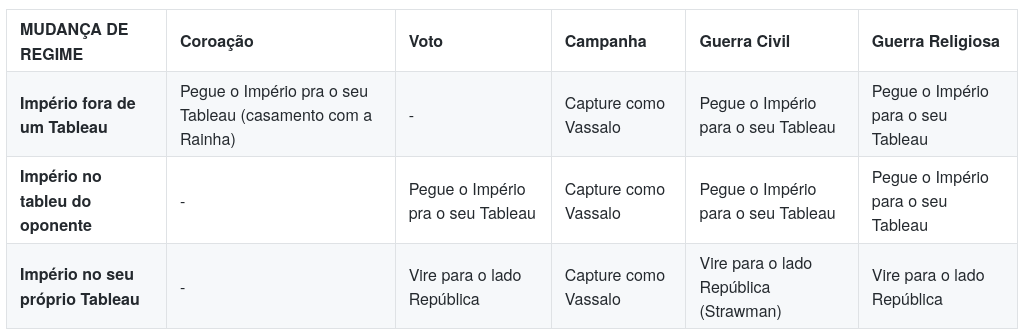
\includegraphics[width=.9\linewidth]{./regime-change.png}
\caption{\label{fig:org993b0e0}
Esta tabela demonstra os efeitos nas mudanças de regime.}
\end{figure}

\subsubsection{REPRESSÃO (REPRIMIR)}
\label{sec:org5a57727}

Remova o Token (não Pirata) do mapa, que é morto, caso o Império não esteja em um Tableau, ou torna-se um token Reprimido na carta do respectivo Império.

\begin{itemize}
\item Caso a repressão seja feita como resultado da colocação de um Agente, pague 1 Florin;

\item Caso seja o resultado da operação de Repressão (\emph{Repress}), ganhe 1 Florin;

\item Caso seja o resultado da operação de Imposto (\emph{Tax}), não há custo;
\end{itemize}


\subsection{\emph{ONE-SHOT} (ÍCONE DA BOMBA)}
\label{sec:org875cd75}

\subsubsection{GUERRAS CIVIS}
\label{sec:org7da11ed}

Existem dois tipos de Guerra Civil: Conspirações e Revolta dos Camponeses (\emph{Peasant Revolt}). Em caso de vitória causam uma Mudança de Regime.

\begin{itemize}
\item \textbf{Conspiração}
\begin{itemize}
\item \textbf{Atacantes:} Todos os Agentes na carta ativa, todos os Cavaleiros e Torres reprimidos naquele Império, e os Piratas na fronteira.
\item \textbf{Defensores:} Cavaleiros e Torres na carta do Mapa. Caso vitória em uma Teocracia, vire a carta para o outro lado.
\end{itemize}

\item \textbf{Revolta dos Camponeses (\emph{Peasant Revolt})}
\begin{itemize}
\item \textbf{Atacantes}: Todos os agentes na carta ativa, todos os Peões (Mercadores) reprimidos naquele Império, seus Mercadores na fronteira e Piratas.
\item \textbf{Defensores}: Cavaleiros e Torres na carta de Mapa.
\end{itemize}
\end{itemize}


\subsubsection{COROAÇÃO}
\label{sec:org44abf1f}

Case a rainha com o Rei de um Império listado no ícone de coroação (pretendentes da rainha), que ainda poderão estar na pilha de Impérios (fora de um Tableau).

A coroação é considerada uma Mudança de Regime.

\begin{itemize}
\item O par Rainha-Rei é tratado como duas cartas separadas durante as Operações do Leste/Oeste, mas é tratado como uma única carta para o movimento (silenciamento) do Bispo.

\item Se não for utilizar a coroação em sua ação, guarde a rainha embaixo da carta do seu personagem, porém adicione o prestígio dela ao seu total no final do jogo, se for o caso.
\end{itemize}

\subsubsection{GUERRAS RELIGIOSAS}
\label{sec:org9a636ec}

Caso jogue uma \textbf{Crusada}, \textbf{Reforma (\emph{Reformation})} ou \textbf{Jihad}, poderá ser iniciada uma Guerra Religiosa naquela localidade.

Uma Guerra Religiosa bem sucedida vira a carta do Mapa para o outro lado da religião especificada e causa uma Mudança de Regime.

\begin{itemize}
\item \textbf{Atacantes}: Todos os Agentes não Bispos na carta ativa, todos os Cavaleiros, Torres e Piratas na fronteira da carta de Mapa da mesma cor dos Agentes da carta jogada, mais quaiquer
\end{itemize}
Cavaleiros nos Impérios adjacentes da mesma cor (esses tokens não se movem).

\begin{itemize}
\item \textbf{Defensores}: Hereges na região, ou seja todos os Cavaleiros, Torres e Piratas de outras cores
\end{itemize}

Uma Guerra Religiosa não pode ser conduzida onde não existam Hereges (inclusives Piratas nas fronteiras). Tokens Reprimidos não contam para essa regra.


\subsubsection{MUDANÇA DE ROTA COMERCIAL}
\label{sec:org44b7f92}

Mova o token de bloqueio da rota (caso exista) cobrindo o respectivo Empório (início da rota) para cobrir e desativar um Empório descoberto da mesma cor.

Essa desativação Reprime qualquer token que possa estar nesse local.

\begin{itemize}
\item Rota da Ilha das Especiarias (\emph{Spice Islands Route}): o jogador deve ter pelo menos um ícone de prestígio de Descoberta em seu Tableau (sem contar a carta sendo jogada) antes de iniciar uma mudança de rota.
\end{itemize}

\subsection{OPERAÇÕES}
\label{sec:org62a165e}

\subsubsection{DECAPITAR (\emph{BEHEAD})}
\label{sec:orgdac29ac}

Descarte uma carta de qualquer Tableau que compartilhe a localização da carta ativa. Todavia uma carta não pode Decapitar a si mesma.

\begin{itemize}
\item Se usada para descartar um Império, a carta usada para Decapitar é também descartada (morta).

\item Regiões (leste/oeste) compartilham localização com cartas de Mapa dessa área. Ex: Região Oeste e Portugal compartilham a mesma localização para efeitos da Decapitação.
\end{itemize}

\subsubsection{CAMPANHA}
\label{sec:org4f36463}

Crie uma batalha em uma carta de Mapa adjacente a localização do Império (inclui diagonais).

\begin{itemize}
\item \textbf{Atacantes}: todos os Cavaleiros na localização do Império;

\item \textbf{Defensores}: Cavaleiros e Torres na carta sendo atacada;
\end{itemize}

Se a Campanha obtiver sucesso o Império sofre uma Mudança de Regime e é reivindicado como Vassalo ao atacante.

\begin{itemize}
\item Custo: pague 1 Florin por Cavaleiro atacante;

\item Essa operação não move os tokens entre as cartas no Mapa;
\end{itemize}

\subsubsection{COMÉRCIO}
\label{sec:orge8668d0}

Pegue um Florin de qualquer carta do mercado especificado.

\subsubsection{CORSÁRIO}
\label{sec:org6a47418}

Mova 1 Pirata da cor especificada para uma fronteira da localização da carta para outra fronteira na mesma localização.

\begin{itemize}
\item Não pode ser movido para uma fronteira com um Pirata de mesma cor;

\item Ao mover-se automaticamente mata qualquer mercador ou Pirata de outra cor;
\end{itemize}

\subsubsection{INQUISIDOR}
\label{sec:org9677dee}

Mova um Bispo da cor especificada de uma carta de um Tableau para uma carta adjacente no mesmo Tableau, ou em uma carta em qualquer Tableau que compartilhe a mesma localização de onde o Bispo está.

\begin{itemize}
\item A presença de de qualquer Bispo em uma carta previne todas as Operações não religiosas de serem usadas (silencia);

\item Se a carta de destino contém um Bispo de qualquer cor, os dois Bispos são mortos;

\item Se a carta de destino possui um token Reprimido, o jogador pode escolher matar um deles sem custo;

\item O Bispo não pode mover-se para a carta de jogador (banqueiro);
\end{itemize}

\subsubsection{REPRIMIR}
\label{sec:orgca11745}

Remova do Mapa um token de determinado tipo na localidade especificada e coloque esse token como um token Reprimido na carta correspondente de Império em jogo.

\begin{itemize}
\item Caso o Império não esteja em jogo, mate o respectivo token e ganhe 1 Florin;
\end{itemize}

\subsubsection{CERCO (\emph{SIEGE})}
\label{sec:orgea7900d}

Mate uma Torre, Cavaleiro ou Pirata na localidade especificada.

\subsubsection{IMPOSTO (\emph{TAX})}
\label{sec:orgc2e0fef}

Mire um mercador na fronteira da localidade especificada. O jogador correspondente deve ou pagar 1 Florin ao Banco (China) ou Reprimir o mercador, então ele deve recrutar (\emph{place a Levy}) no Império taxado
(não é possível utilizar essa opção caso o Império esteja saturado).

\subsubsection{VOTO}
\label{sec:org23c737f}

Causa uma mudança de Regime em um Império. O Império deve estar em um Tableau mas não como Vassalo e do lado especificado (leste/oeste).

\begin{itemize}
\item Custo: pague 1 Florin por token Reprimido no Império;

\item Para executar essa operação o jogador deve possuir mais mercadores do que qualquer outro jogador na fronteira desse Império.
\end{itemize}
\end{document}
